\documentclass{standalone}
\usepackage{pgfplots}
\pgfplotsset{compat=1.18}

\begin{document}

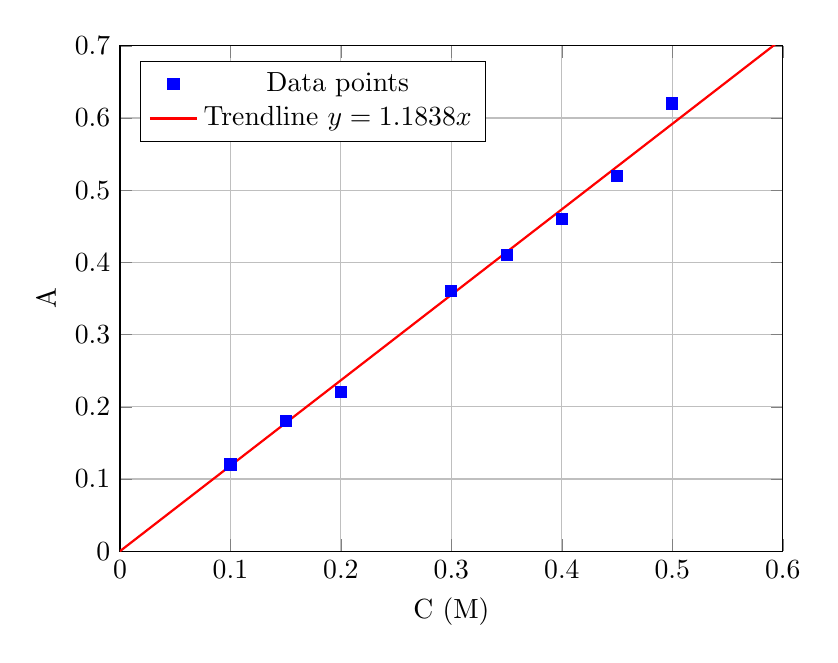
\begin{tikzpicture}
    \begin{axis}[
        xlabel={C (M)},
        ylabel={A},
        grid=both,
        xmin=0, xmax=0.6,
        ymin=0, ymax=0.7,
        legend pos=north west,
        width=10cm, height=8cm
    ]

    % Plot data points
    \addplot[
        only marks,
        mark=square*,
        color=blue,
    ] coordinates {
        (0.1, 0.12)
        (0.15, 0.18)
        (0.2, 0.22)
        (0.3, 0.36)
        (0.35, 0.41)
        (0.4, 0.46)
        (0.45, 0.52)
        (0.5, 0.62)
    };
    \addlegendentry{Data points}

    % Plot trendline y=1.1838x
    \addplot[
        domain=0:0.6,
        color=red,
        thick
    ] {1.1838 * x};
    \addlegendentry{Trendline $y=1.1838x$}

    \end{axis}
\end{tikzpicture}

\end{document}